\documentclass[11pt,fleqn]{article} 
\usepackage[margin=0.8in, head=0.8in]{geometry} 
\usepackage{amsmath, amssymb, amsthm}
\usepackage{fancyhdr} 
\usepackage{palatino, url, multicol}
\usepackage{graphicx} 
\usepackage[all]{xy}
\usepackage{polynom} 
\usepackage{pdfsync}
\usepackage{enumerate}
\usepackage{framed}
\usepackage{setspace, adjustbox}
\usepackage{array%,tikz, pgfplots
}

\usepackage{tikz, pgfplots}
\usetikzlibrary{calc}
\pgfplotsset{my style/.append style={axis x line=middle, axis y line=
middle, xlabel={$x$}, ylabel={$y$}, axis equal }}

\pagestyle{fancy} 
\lfoot{UAF Calculus I}
\rfoot{2-6 Limits at Infinity}


\newcommand{\be}{\begin{enumerate}}
\newcommand{\ee}{\end{enumerate}}

\newcommand{\bi}{\begin{itemize}}
\newcommand{\ei}{\end{itemize}}

\begin{document}
\setlength{\parindent}{0cm}
\renewcommand{\headrulewidth}{0pt}
\newcommand{\blank}[1]{\rule{#1}{0.75pt}}
\renewcommand{\d}{\displaystyle}
\vspace*{-0.7in}
\begin{center}
  \LARGE \sc{Section 2-6 Limits at Infinity (day 1)}
\end{center}

\begin{enumerate}

%
%\item  Sketch a graph of $y = \tan^{-1} x$ and find the $\d \lim_{x \to \infty} \tan^{-1} x$ and $\d \lim_{x \to -\infty} \tan^{-1} x$. 
%
%\vskip2.5in
%
%\textbf{Example 2:}

\item Consider the function $f(x)$ whose graph is shown below. %Find the infinite limits, limits at infinity, and asymptotes for the function $f$ whose graph is shown below. 
%
%\begin{quote}
%  \begin{flushleft}
%    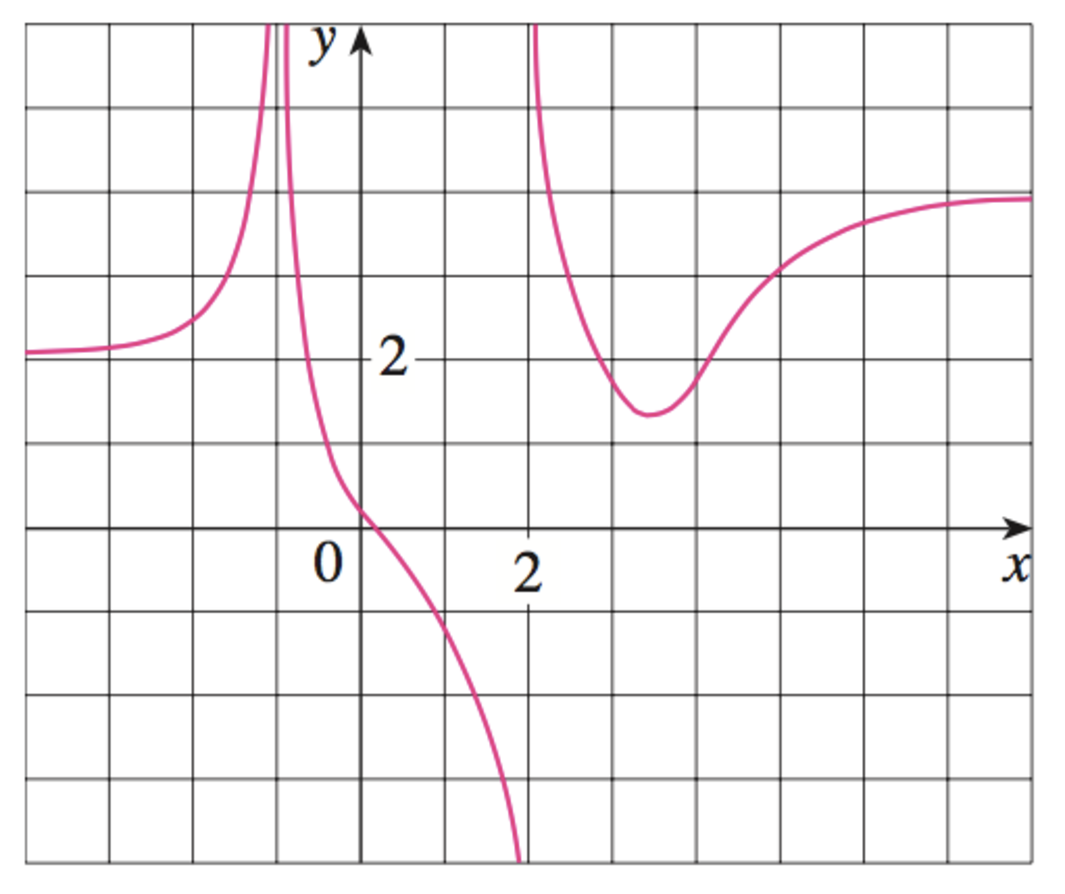
\includegraphics[width=2.25in]{limits-at-infinity}
%  \end{flushleft}
%\end{quote}
%
%\newpage
%\vspace*{-0.75in}


%
\begin{adjustbox}{valign=t,minipage={.4\textwidth}}
\begin{center}

    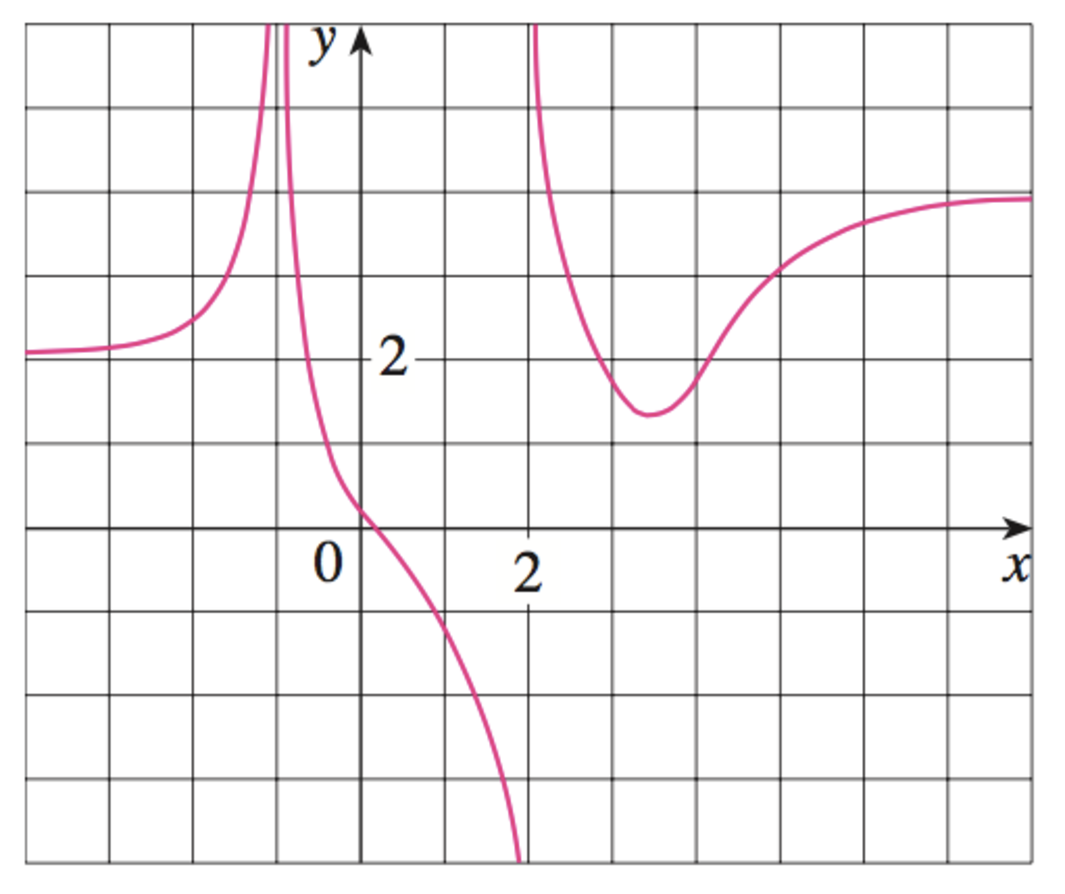
\includegraphics[width=2.75in]{limits-at-infinity}

 \end{center}
\end{adjustbox}
%
%
\begin{adjustbox}{valign=t,minipage={.45\textwidth}}
\begin{center}
\begin{enumerate}
   \item Determine the following limits from the graph:
    
   \begin{enumerate}
   \item $\displaystyle{\lim_{x\to 2^{-}} f(x) = }$
   
   \item $\displaystyle{\lim_{x\to 2^{+}} f(x) = }$
   
    \item $\displaystyle{\lim_{x\to -1^{-}} f(x) = }$
   
   \item $\displaystyle{\lim_{x\to -1^{+}} f(x) = }$
   
     \item $\displaystyle{\lim_{x\to 2.5} f(x) = }$
   
      \item $\displaystyle{\lim_{x\to \infty} f(x) = }$
      
         \item $\displaystyle{\lim_{x\to -\infty} f(x) = }$
         
         \ee
         
 
 \ee
\end{center}
\end{adjustbox}

\be[(b)]%oh so hacky.
    \item Write the equations of any horizontal and vertical asymptotes.
    \ee
     
     \vspace{.7cm}


\item By thinking about the graphs of these functions or using your intuition (what's happening as $x$ gets big?), find the following limits, if they exist. 

  \begin{multicols}{3}{
      % make sure you added \usepackage{enumerate}
      \vspace*{-0.45in}
      \begin{enumerate}[a)]
       \item $\d \lim_{x \to \infty} \frac{1}{7x + 1}$
      \item $\d \lim_{x \to \infty} \sin x$
      \item $\d \lim_{x \to \infty} 3 e^{-x}$
      \end{enumerate}}
  \end{multicols}
%
\vskip0.7in
%

\item Explain: as $x \to \infty$, what happens to $\d{\frac{1}{x}}$? Why? What happens to $\d \frac{1}{x^{n}}$ for any positive integer $n$?

\vspace{.7in}


\begin{framed}
  \textbf{How to Determine Limits at Infinity for rational functions:} Divide each term in the the numerator
  and denominator by the highest power of $x$ in the denominator. \end{framed}
%
%
\item  Find the limit.
 \vspace*{-0.15in}
  \begin{multicols}{2}
      \vspace*{-0.45in}
    \begin{enumerate}
    \item $\d \lim_{x \to \infty} \frac{2x + 5}{x-4}$ (highest power is $x$)
    
    \vspace{1cm}
    
    \item $\d \lim_{x \to \infty} \frac{x+4}{x^2 + x - 3}$ (highest power is $x^{2}$)

    \vspace{1cm}


\ee
\end{multicols}

\newpage

\item Find the following limits.
\be
 \item $\d \lim_{x \to \infty} \frac{2x^2+5}{3x^2 + 1}$
 

\vfill
 
         \item $\d \lim_{x \to \infty} \frac{2x+5}{3x^2 + 1}$
         
      
\vfill
         
         
     \item $\d \lim_{x \to \infty} \frac{2x^3+5}{3x^2 + 1}$
     
     \vfill
    \end{enumerate}
 
 
 \item 
 \be \item Sketch a graph of a function $f(x)$ that has the following properties:
 
 \begin{adjustbox}{valign=t,minipage={.45\textwidth}}
 \begin{tikzpicture}[scale = .6]
 \draw[ultra thin] (-5, -5) grid (7,7);
 \draw[<->, ultra thick] (-5.5,0) -- (7.5,0);
  \draw[<->, ultra thick] (0, -5.5) -- (0, 7.5);

 \end{tikzpicture}
 \end{adjustbox}
 %
  \begin{adjustbox}{valign=t,minipage={.55\textwidth}}

\smallskip
% \begin{multicols}{1}
 \be \item $f(0) = 3$ 
 
 \item $\d\lim_{x\to 0^{-}} f(x) = 4$
 
 \item $\d\lim_{x\to 0^{+}} f(x) = 2$
 
  \item $\d\lim_{x\to \infty} f(x) = 3$
  
    \item $\d\lim_{x\to -\infty} f(x) = -\infty$
    
     \item $\d\lim_{x\to 4^{-}} f(x) = -\infty$
 
 \item $\d\lim_{x\to 4^{+}} f(x) = \infty$
 \ee
% \end{multicols} 
  \end{adjustbox}
 
 \smallskip
 
 \item List the equation(s) of any horizontal asymptotes \hrulefill
 
 \item List the equation(s) of any vertical asymptotes \hrulefill
 
 \item List any real numbers where $f$ is not continuous \hrulefill
 \ee
  

  
  \newpage
%  
%  %\fbox{DAY 2: Sometimes we have to use tricks!}
%  \begin{center}
%  \LARGE \sc{Section 2-6 Limits at Infinity (day 2):\\Sometimes we have to use tricks!}
%\end{center}
%  
%  \item  Multiply the top and bottom by $\frac{1}{e^{x}}$, to help compute:
%  
%    $\d \lim_{x \to \infty} \frac{1 + 5e^x}{7 - e^x}$ 
%    
%\vfill    
%    \item This time we need two tricks: (1) rewrite the difference of natural logs as a quotient, and (2) use the continuity of natural log to pull it through the limit, to help compute:
%    
%    $\d \lim_{x \to \infty} [ \ln (2 + x) - \ln (1+x) ]$
%    
%    \vfill
%    
%    \item 
%    
%    \item  Even though the $x^{6}$ is part of a term in the square root, as $x$ blows up, $\sqrt{x^{6} + ...}$ ``looks like'' $x^{3}$. So try multiplying the top and bottom by $\frac{1}{x^{3}}$ (which is the same as $\sqrt{\frac{1}{x^{6}}}$).
%    
%     $\d \lim_{x \to \infty} \frac{\sqrt{3x^6-x}}{x^3 + 1}$
%     
%     \vfill
%     
%     
%     \item If, when you think about a limit, it ``looks like'' $\infty - \infty$, that means you need to do more work.     
%     $\d \lim_{x \to \infty} (\sqrt{x^2+1} - x)$
%     
%     \vfill
%     
%     
%  \item We know that $-1 \leq \cos(x) \leq 1$. Use that fact plus the \emph{Squeeze Theorem} to evaluate the following:
%  
%    $\d \lim_{x \to \infty} e^{-2x} \cos x$
%    \vfill
%
%\vskip2.5in
%\textbf{Example 4:} Evaluate the following limits. 
%
%  \begin{multicols}{3}{
%      % make sure you added \usepackage{enumerate}
%      \vspace*{-0.45in}
%      \begin{enumerate}[(a)]
%     \item $\d \lim_{x \to \infty} \frac{2x^2+5}{3x^2 + 1}$
%          \item $\d \lim_{x \to \infty} \frac{2x+5}{3x^2 + 1}$
%     \item $\d \lim_{x \to \infty} \frac{2x^3+5}{3x^2 + 1}$
%      \end{enumerate}}
%  \end{multicols}
%
%
%\vskip2.5in
%\newpage
%\vspace*{-1in}
%\textbf{Example 5:} Find the following limits at infinity. 
%
%  \begin{multicols}{2}{
%      % make sure you added \usepackage{enumerate}
%      \vspace*{-0.45in}
%      \begin{enumerate}[(a)]
%      \item $\d \lim_{x \to \infty} \frac{1 + 5e^x}{7 - e^x}$
%      \item $\d \lim_{x \to \infty} [ \ln (2 + x) - \ln (1+x) ]$
%      \end{enumerate}}
%  \end{multicols}
%
%\vskip2in
%
%\textbf{Example 6:} Find the limit. 
%
%  \begin{multicols}{2}{
%      % make sure you added \usepackage{enumerate}
%      \vspace*{-0.45in}
%      \begin{enumerate}[(a)]
%  \item[(a)] $\d \lim_{x \to \infty} \frac{x + 2}{\sqrt{9x^2+1}}$ 
%  \item[(b)] $\d \lim_{x \to \infty} \frac{\sqrt{3x^6-x}}{x^3 + 1}$
%      \end{enumerate}}
%  \end{multicols}
%
%\vskip2.7in
%
%\begin{framed}
%  \textbf{How do deal with limits as $x \to - \infty$}: Replace $x$ by
%  $-x$ and take the limit as $x \to \infty$.
%\end{framed}
%
%\textbf{Example 7:} Find the limit.
%
%  \begin{multicols}{2}{
%      \vspace*{-0.45in}
%    \begin{enumerate}
%    \item[(a)] $\d \lim_{x \to -\infty} \frac{2x}{\sqrt{x^2 +2}}$ \vskip2in
%    \item[(b)] $\d \lim_{x \to -\infty} (5 - 3 e^x)$
%    \end{enumerate}}
%  \end{multicols}
%
%\newpage
%
%\textbf{Example 8:} Evaluate the following limits. 
%
%
%  \begin{multicols}{2}{
%    \begin{enumerate}
%      \vspace*{-0.45in}
%    \item[(a)] $\d \lim_{x \to \infty} (\sqrt{x^4 + 6x^2} - x^2)$
%      \vskip3in
%    \item[(b)] $\d \lim_{x \to \infty} (\sqrt{x^2+1} - x)$
%    \end{enumerate}}
%  \end{multicols}
%
%\vskip4.2in
%
%\textbf{Example 9:} Evaluate the following limits. 
%
%  \begin{multicols}{2}{
%      % make sure you added \usepackage{enumerate}
%      \vspace*{-0.45in}
%      \begin{enumerate}[(a)]
%      \item $\d \lim_{x \to 0^-} e^{1/x}$
%      \item $\d \lim_{x \to \infty} e^{-2x} \cos x$
%      \end{enumerate}}
%  \end{multicols}
%
%
%\newpage
%
%
%
%
%
%
%
%
%
%
%
%\textbf{Example 11:} Sketch the graph of $y = (x-2)^4 (x+1)^3 (x-1)$
%by finding its intercepts and its limits as $x \to \pm \infty$. 
%\vskip0.25in
%
%\begin{tikzpicture}[scale=0.95][>=latex]
%%x axis
%\draw[->] (-4 ,0) -- (4 ,0) node[below] {$x$};
%\foreach \x in {-3,...,3}
%\draw[shift={(\x,0)}] (0pt,2pt) -- (0pt,-2pt);
%%y axis
%\draw[->] (0,-4) -- (0,4) node[left] {$y$};
%\foreach \y in {-3,...,3}
%\draw[shift={(0,\y)}] (2pt,0pt) -- (-2pt,0pt);
%% \node[below left] at (0,0) {\footnotesize $0$};
%\end{tikzpicture}
%
%\vskip1.5in
%
%\textbf{Example 12:} Find the horizontal and vertical asymptotes of $\d f(x) = \frac{\sqrt{16x^2 + 1}}{2x - 8}$.

\ee
\end{document}